\documentclass[tikz]{standalone}
\usepackage{amsmath}
\usepackage{amssymb}
\begin{document}
	
	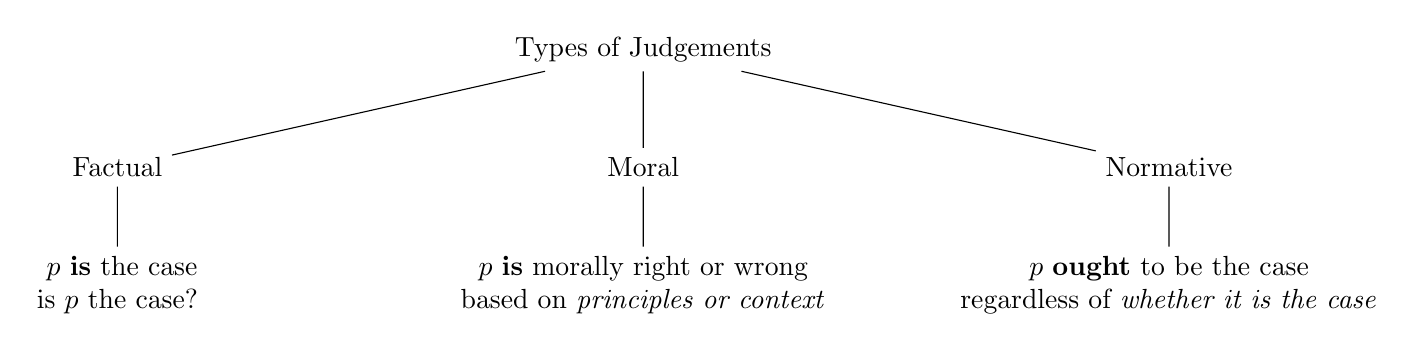
\begin{tikzpicture}[every node/.style={align=center},level 1/.style={sibling distance=19em},level 2/.style={sibling distance=40mm}, level 3/.style={sibling distance=35mm}]
		\node {Types of Judgements}
		[sibling distance=7cm]
		child { node {Factual} 
			child { node { \ \textit{$p$} \textbf{is} the case \\ is \textit{$p$} the case?}} } % Clarified factual branch
		child { node {Moral}  % Replaced placeholder
			child { node {\textit{$p$} \textbf{is} morally right or wrong \\ based on \textit{principles or context}} }} % Added moral node
		child { node {Normative} 
			child{ node {\textit{$p$} \textbf{ought} to be the case \\ regardless of \textit{whether it is the case}} }} % Clarified normative branch
		; % End of diagram
	\end{tikzpicture}
	
\end{document}
